% Tipe dokumen adalah report dengan satu kolom. 
% Menggatur setting halaman 
\documentclass[12pt, a4paper, onecolumn, oneside, final]{report}

% Load konfigurasi LaTeX untuk tipe laporan thesis
\usepackage{unpam}
\usepackage{enumitem}
\usepackage{array}
\usepackage{graphics}
\usepackage{microtype}
\usepackage{adjustbox}
\usepackage[numbers]{natbib}


% Daftar pemenggalan suku kata dan istilah dalam LaTeX
%
% Hyphenation untuk Indonesia 
%
% @author  Enggar Alfianto
% @version 1.00
% 
% Tambahkan cara pemenggalan kata-kata yang salah dipenggal secara otomatis 
% oleh LaTeX. Jika kata tersebut dapat dipenggal dengan benar, maka tidak 
% perlu ditambahkan dalam berkas ini. Tanda pemenggalan kata menggunakan 
% tanda '-'; contoh:
% menarik
%   --> pemenggalan: me-na-rik
%

\hyphenation{
    % alphabhet A
    a-na-li-sa a-tur
    a-pli-ka-si
    a-na-li-tik
    % alphabhet B
    ba-ngun-an
    be-be-ra-pa
    ber-ge-rak
    ber-ke-lan-jut-an
    ber-pe-nga-ruh
    bim-bing-an
    % alphabhet C
    ca-ri
    % alphabhet D
    di-sim-pan di-pim-pin de-ngan da-e-rah di-ba-ngun da-pat di-nya-ta-kan
    di-sim-bol-kan di-pi-lih di-li-hat de-fi-ni-si
    di-rahmat-i
    di-identifi-kasi-kan
    di-re-pre-sen-ta-si-kan
    du-kung-an-nya
    % alphabhet E
    e-ner-gi eks-klu-sif
    % alphabhet F
    fa-si-li-tas
    fe-no-me-na
    % alphabhet G
    ga-bung-an ge-rak
    % alphabhet H
    ha-lang-an
    hamilton-nia-nya
    % alphabhet I
    % alphabhet J
    % alphabhet K
    ke-rapat-an
    ke-hi-lang-an
    ku-ning
    kompu-tasi
    kua-li-tas ka-me-ra ke-mung-kin-an ke-se-pa-ham-an
    % alphabhet L
    ling-kung-an
    % alphabhet M
    me-nge-luar-kan
    me-neng-ah
    mem-perhitung-kan
    mem-ban-ding-kan
    meng-a-tas-i me-mung-kin-kan me-nge-na-i me-ngi-rim-kan
    meng-u-bah meng-a-dap-ta-si me-nya-ta-kan mo-di-fi-ka-si
    meng-a-tur
    micro-service
    % alphabhet N
    nya-ta non-eks-klu-sif
    nano-tekno-logi
    % alphabhet O
    % alphabhet P
    pa-ling
    pe-nye-rap-an
    pe-ngon-trol
    pe-mo-del-an
    pe-ran  pe-ran-an-nya
    pem-ba-ngun-an pre-si-den pe-me-rin-tah prio-ri-tas peng-am-bil-an
    peng-ga-bung-an pe-nga-was-an pe-ngem-bang-an
    pe-nga-ruh pa-ra-lel-is-me per-hi-tung-an per-ma-sa-lah-an
    pen-ca-ri-an peng-struk-tur-an
    % alphabhet Q
    % alphabhet R
    ran-cang-an
    % alphabhet S
    si-mu-la-si sa-ngat
    se-bagai
    semi-konduktor
    % alphabhet T
    te-ngah
    ter-da-pat
    ter-selesai-kanya
    % alphabhet U
    % alphabhet V
    % alphabhet W
    % alphabhet X
    % alphabhet Y
    % alphabhet Z
    % special
}

% Variabel baru untuk menyimpan nomor halaman
\newcounter{originalpagenumber}%

% Awal bagian penulisan laporan
\begin{document}

% Sampul Laporan
\begin{titlepage}
\begin{center}
	\onehalfspacing
	\large \bfseries \textit{AutomaticDeployment}  Aplikasi berbasis \textit{Microservice} Pada Platform Kubernetes Dengan Metode \textit{Pull Up Based} \\
	\vspace{1cm}
	 \large Proposal Tugas Akhir \\
	\vspace{0.5cm}
	
	{\small \normalfont Diajukan Untuk Memenuhi\\
	Persyaratan Guna Meraih Gelar Sarjana\\
	Informatika Universitas Muhammadiyah Malang}
	\vspace{2cm}
	
	
\includegraphics[width=6cm]{images/logo_umm.png}
	
	\vspace{1cm}
	Muhammad Zein Ihza Fahrozi \\
	201810370311072 \\
	
	\vspace{3cm}
	
	\normalsize PROGRAM STUDI TEKNIK INFORMATIKA FAKULTAS TEKNIK \\
	UNIVERSITAS MUHAMMADIYAH MALANG \\
	2021
	

	
\end{center}

\end{titlepage}

\newpage

% Daftar isi, gambar, dan tabel
% Gunakan penomeran Romawi (i, ii, iii, ...) setelah bagian ini.

\pagenumbering{roman}

% Judul Laporan
% \begin{center}
	\onehalfspacing
	\large \bfseries PERANCANGAN SISTEM INFORMASI KOPERASI SIMPAN PINJAM BERBASIS WEB \\
	\vspace{1cm}
	 \large SKRIPSI \\
	 \normalsize Diajukan Untuk Melengkapi Salah Satu Syarat \\ Memperoleh Gelar Sarjana Komputer
	
	\vspace{2cm}
	
	\includegraphics[width=6cm]{images/logo-unpam.png}
	
	\vspace{1cm}
	\large OLEH: \\
	IMRON ROSDIANA \\
	2010140419
	
	\vspace{3cm}
	
	\normalsize PROGRAM STUDI TEKNIK INFORMATIKA \\
	\large FAKULTAS TEKNIK \\
	UNIVERSITAS PAMULANG \\
	2014
	

	
\end{center}

\newpage

% Lembar Pernyataan
%\phantomsection \addcontentsline{toc}{chapter}{LEMBAR PERNYATAAN}
%%
% Lembar pengesahan Naskah

\chapter*{\uppercase{LEMBAR PERNYATAAN}}
\vspace{1cm}

\noindent Yang bertanda tangan di bawah ini:
\renewcommand{\arraystretch}{1.5}
\begin{table}[ht]
\begin{adjustwidth}{-0.15cm}{}
	\begin{tabular}{lll}
		Nama & : & Imron Rosdiadna \\
		NIM & : & 2010140419 \\
		Program Studi & : & Teknik Informatika \\
		Fakultas & : & Teknik \\
		Jenjang Pendidikan & : & Strata 1
	\end{tabular}
\end{adjustwidth}
\end{table} \\

\vspace{-1cm}
\noindent Menyatakan bahwa skripsi yang saya buat dengan judul:

\vspace{0.3cm}
\noindent PERANCANGAN SISTEM INFORMASI KOPERASI SIMPAN PINJAM BERBASIS WEB
\begin{enumerate}[nolistsep,leftmargin=0.5cm]
	\item Merupakan hasil karya tulis ilmiah sendiri, bukan merupakan karya yang pernah diajukan untuk memperoleh gelar akademik oleh pihak lain, dan bukan merupakan hasil plagiat.
	\item Saya ijinkan untuk dikelola oleh Universitas Pamulang sesuai dengan norma dan etika yang berlaku.
\end{enumerate}
Pernyataan ini saya buat dengan penuh tanggung jawab dan saya bersedia menerima konsekuensi apapun sesuai aturan yang berlaku apabila dikemudian hari pernyataan ini tidak benar.

\vspace{2cm}
\begin{table}[ht]
\begin{adjustwidth}{-0.15cm}{}
	\begin{tabular}{l}
	Pamulang, 01 Agustus 2014 \\[2cm]
	(Nama Orang)
	\end{tabular}
\end{adjustwidth}	
\end{table}

\newpage

% Lembar Persetujuan
\phantomsection \addcontentsline{toc}{chapter}{LEMBAR PERSETUJUAN}
%
% Lembar persetujuan

\doublespacing
\chapter*{\uppercase{LEMBAR PERSETUJUAN}}
\onehalfspacing
\begin{center}
	\large \bfseries \textit{AutomaticDeployment}  Aplikasi berbasis \textit{Microservice} Pada Platform Kubernetes Dengan Metode \textit{Pull Up Based} \\

	\vspace{2.5cm}

	\bfseries{Muhammad Zein Ihza Fahrozi\\
		201810370311072}

	\vspace{1cm}
	\normalfont\normalsize Telah Direkomendasikan Untuk Diaujan Sebagai\\
	Judul Tugas Akhir Di\\
	Program Studi Informatika Universitas Muhammadiyah Malang
\end{center}

\vspace{5cm}



\newcolumntype{P}[1]{>{\centering\arraybackslash}p{#1}}
\newcolumntype{M}[1]{>{\centering\arraybackslash}m{#1}}

\begin{center}
	\normalfont\normalsize Malang, \today \\
	Menyetujui,
\end{center}

% \renewcommand{\arraystretch}{1} % Default value: 1
% \setlength{\tabcolsep}{10pt}
\begin{table}[!ht]
	\centering
	\begin{tabular}{M{7cm}M{7cm}}

		Dosen I                                                                                             & Dosen II                                                                                        \\
		\rule{0pt}{4cm} \bfseries{\underline{Agus Eko Minarno, S.Kom., M.Kom.}} \newline NIP. 108.1410.0540 & \rule{0pt}{4cm} \bfseries{\underline{Ilyas Nuryasin S.Kom, M.Kom.}} \newline NIP. 108.1410.0561 \\
	\end{tabular}
\end{table}

\newpage
\onehalfspacing

% Lembar Pengesahan
%\phantomsection \addcontentsline{toc}{chapter}{LEMBAR PENGESAHAN}
%%
% Lembar persetujuan
\doublespacing
\chapter*{\uppercase{LEMBAR PENGESAHAN}}

\renewcommand{\arraystretch}{1.5}
\begin{table}[ht]
\begin{adjustwidth}{-0.15cm}{}
	\begin{tabularx}{\textwidth}{llX}
		Nama & : & Imron Rosdiadna \\
		NIM & : & 2010140419 \\
		Program Studi & : & Teknik Informatika \\
		Fakultas & : & Teknik \\
		Jenjang Pendidikan & : & Strata 1 \\
		Judul Skripsi & : & PERANCANGAN SISTEM INFORMASI KOPERASI SIMPAN PINJAM BERBASIS WEB
	\end{tabularx}
\end{adjustwidth}
\end{table}

\onehalfspacing
\noindent Skripsi ini telah dipertahankan dihadapan dewan penguji ujian Skripsi Fakultas Teknik, Program Studi Teknik Informatika dan dinyatakan LULUS. \\
Pamulang, 01 Agustus 2014

\noindent
\vspace{0.3cm}
\begin{tabularx}{\linewidth}{XX}
\begin{minipage}{\linewidth}\centering
\vspace{2cm}
\underline{Penguji 1}\\
Penguji 1
\end{minipage} &
\begin{minipage}{\linewidth}\centering
\vspace{2cm}
\underline{Penguji 2}\\
Penguji 2
\end{minipage}
\end{tabularx}

\vspace{2.5cm}
\begin{center}
\begin{minipage}{\linewidth}\centering
\underline{Pembimbing, S.Kom, M, Kom} \\
Pembimbing \\
\vspace{1cm}
Mengeetahui, \\
\vspace{2.5cm}
\underline{Kaprodi, S.Si, M.Si} \\
KaProdi Teknik Informatika
\end{minipage}
\end{center}

\newpage
\onehalfspacing

% Lembar Abstract
% \phantomsection \addcontentsline{toc}{chapter}{ABSTRACT}
% %
% Halaman Abstract

\chapter*{ABSTRACT}

\begin{singlespace}
\blindtext \\[20pt]
Keywords: \textit{Information System, Testing Project}
\end{singlespace}

\newpage

% Lembar Abstrak
% \phantomsection \addcontentsline{toc}{chapter}{ABSTRAK}
% %
% Halaman Abstrak

\chapter*{ABSTRAK}

\begin{singlespace}
\blindtext \\[20pt]
Keywords: \textit{Sistem Informasi, Testing Project}
\end{singlespace}

\newpage

% Kata Pengantar
% \phantomsection \addcontentsline{toc}{chapter}{KATA PENGANTAR}
% % Kata Pengantar
\chapter*{KATA PENGANTAR}

\blindtext \\[2cm]

\hfill
\begin{minipage}[t]{4.9cm}
\centering
	Pamulang, 01 Agustus 2014 \\ [2cm]
	Imron Rosdiana
\end{minipage}

\newpage

% \vspace*{-2.5cm}
% \tableofcontents
% \phantomsection
% \addcontentsline{toc}{chapter}{DAFTAR ISI}
% \clearpage
% \vspace*{-2.5cm}
% \listoftables
% \phantomsection
% \addcontentsline{toc}{chapter}{DAFTAR TABEL}
% \clearpage
% \vspace*{-2.5cm}
% \listoffigures
% \phantomsection
% \addcontentsline{toc}{chapter}{DAFTAR GAMBAR}
% \clearpage

% Gunakan penomeran Arab (1, 2, 3, ...) setelah bagian ini.
\pagenumbering{arabic}

%
% Atur header dan footer dalam dokumen.
% 
\renewcommand{\headrulewidth}{0.0pt}
\fancyhf{}
\fancyhead[L]{}
\fancyhead[C]{}
% \fancyhead[R]{\thepage}
\fancyfoot[CE,CO]{\thepage}
\renewcommand{\headrulewidth}{0.0pt}
\renewcommand{\footrulewidth}{0.0pt}
\pagestyle{fancy}

\onehalfspacing
%-----------------------------------------------------------------------------%
\chapter{PENDAHULUAN}
%-----------------------------------------------------------------------------%

\vspace{4.5pt}
\setlength{\parskip}{0.5em}

\section{Latar Belakang} \label{sec:latar_belakang}
Sebuah perangkat lunak sebelum digunakan oleh pengguna secara luas perlu dilakukan proses deployment
pada perangkat lunak tersebut. Deployment sebuah perangkat lunak dapat didefinisikan sebagai akusisi
dan eksekusi sebuah perangkat lunak. Proses ini biasanya dilakukan oleh seorang software deployer atau dalam bahasa yang sering
digunakan belakangan ini seorang SRE (site reliability engineer)\cite{Lyu2007}.
Maka dari itu dapat dikatan deployment adalah aktivitas post-production sebuah perangkat lunak untuk digunakan oleh konsumen.
Proses deployment sebuah perangkat lunak terdiri dari beberapa proses yang saling berhubungan seperti proses release sebuah perangkat lunak,
instalasi perangkat lunak kedalam environment exectuion, dan aktivasi sebuah software\cite{Carzaniga1998}.

Untuk mendeploy sebuah sistem perangkat lunak juga ada beberapa yang harus diperhatikan antara lain sub-komponen yang dibutuhkan atau package external,
resource (hardware). Untuk melakukan deploymen sub-komponen ini dibutuhkannya sebuah konfigurasi yang mendeskripsikan versi sub-komponen yang digunakan oleh perangkat lunak.
Dengan bahasa modern sekarang konfigurasi sub-komponen yang digunakan oleh main aplikasi biasanya sudah automatis terbuat contohnya antara lain adalah;
go modules\cite{go_mod} dalam bahasa Golang, requirement file\cite{requirementPython} dalam bahasa Python, atau file RubySpec\cite{rubySpec} pada bahasa Ruby.
\par
Terdapat beberapa karakteristik yang mendasar pada deployment sebuah perangkat lunak yang ditulis oleh Alan Dearle yaitu\cite{Dearle2007};
\textbf{\textit{Release}} berupa jembatan antara proses deployment dengan proses development. yang meliputi semua operasi
yang diperlukan untuk mempersiapkan sebuah sistem  untuk di-transfer ke konsumen.
Aktivitas release ini juga menentukan resource yang dibutuhkan oleh sebuah sistem perangkat lunak untuk dapat beroperasi pada environment nya.
Setelah itu dilakukan packaging pada sistem perangkat lunak.
Package tersebut harus mengandung komponen yang dibutuhkan oleh sistem, deskripsi sistem, dependencies pada komponen eksternal, prosedur deployment,
dan semua informasi yang relevan dari sistem tersebut pada environment yang akan dijalankan.
\textbf{\textit{Installation}} diperlukan untuk persiapan melakukan activation. \textbf{\textit{Activation}} adalah proses ekseksui sebuah perangkat lunak pada waktu tertentu, biasa menggunakan grafik antar muka ataupun proses daemon.
Updating adalah proses untuk mengganti bagian dari perangkat lunak yang terinstal dengan versi yang lebih baru.
Selanjutnya yaitu \textbf{\textit{Undeployment}} yaitu proses menghapus software yang terinstall dalam sebuah mesin ini dapat disebut dengan \textit{deinstallation}.
\par
Menurut Mockus dkk\cite{Mockus2005} kualitas deployment sebuah perangkat lunak masuk kedalam faktor utama dalam persepsi konsumer dalam hal kualitas sebuah perangkat lunak.
Jansen dan Brinkkemper\cite{Jansen2006} juga mengatakan bahwa kelancaran sebuah deployment perangkat lunak adalah hal esensial untuk meningkatkan produk perangkat lunak sebuah perusahaan/organisasi.
Tetapi terdapat beberapa tantangan yang dihadapi pada saat melakukan aktivitas deploymet.
Menurut Antonio Carzaniga\cite{Carzaniga1998} terdapat beberapa tantangan yang sering dihadapi pada saat melakukan deployment yaitu;
\textbf{Mengganti} atau melakukan update sebuah sistem terhadap komponen yang sudah berjalan,
\textbf{Dependencies} komponen antar satu sama lain, dan
\textbf{Koordinasi} ketika melakukan update apakah akan mengganggu proses bisnis yang sedang berjalan atau tidak, dan juga
\textbf{Mengatur} platform yang heterogen misalnya terhadap spesifik sistem operasi yang digunakan.
\par
Seiring berjalannya waktu, sebuah aplikasi cenderung menjadi semakin  kompleks\cite{Tania2014, Newman2015}.
Dengan team pengembang dan aplikasi yang selalu bertumbuh  dari sisi kompleksitas dan \textit{maintainability} biasanya
menyebabkan model  pengembangan aplikasi menjadi susah untuk dikembangkan atau dapat dikatakan  terdapat \textit{bottleneck}
sehingga aplikasi menjadi tidak efisien\cite{Yale2016}. Dengan berkembangnya kompleksitas sebuah aplikasi diperlukan
sebuah arsitektur yang  bisa menyelesaikan hal itu, salah satu caranya yaitu menggunakan arsitektur \textit{microservice}\cite{Tania2014}.
Dengan \textit{microservice} aplikasi dibagi menjadi bagian-bagian kecil (unit) yang terpisah satu dengan lainnya\cite{Tania2014}.
Masing-masing bagian aplikasi ini  dapat dijalankan dan dikembangkan secara independent (dari sisi developer)\cite{Xiao2017}.
\par
Saat ini aplikasi berbasis \textit{microservice} menjadi pilihan sebagai arsitektur utama ketika
membangun aplikasi yang scalable\cite{Wu2014}. Aplikasi berbasis \textit{microservice} ini
dulunya dikembangkan dengan dengan menjalankan beberapa VM  (virtual machine)
yang saling berkomunikasi satu sama lain melalui REST/HTTP  (Hypertext Transfer Protocol)
ataupun RPC \textit{(Remote Procedure Call)}\cite{Khazaei2016}. Karena  pada saat itu deployment \textit{microservice} itu sendiri
masih berbasis VM yang  membutuhkan operasi manual dan juga biaya yang mahal, aplikasi berbasis
\textit{microservice} pun menjadi susah dan kompleks dari sisi biaya dan waktu yang  dibutuhkan untuk dilakukan
pengembangan dan juga \textit{scaling}\cite{Khazaei2016} .
\par
\newpage
Teknologi VM sendiri sudah perlahan ditinggalkan ketika merancang \textit{microservice}.
Dengan adanya teknologi \textit{containerization} aplikasi dapat dibungkus agar dapat dijalankan dengan mudah dan efisien \cite{Khazaei2016}.
Menjalankan aplikasi dengan  abstraksi yang diberikan oleh sebuah \textit{container} juga membawa fleksibilitas
dalam  pengelolaannya. Salah satu manfaatnya adalah scaling aplikasi yang jauh lebih  mudah, yaitu hanya
dengan melakukan penyesuaian jumlah \textit{container} yang  dijalankan\cite{Singh2017}.
\par
\textit{Containerization}\cite{davidbritch} ini sangat berdampak pada aspek infrastruktur dan \textit{runtime} sebuah aplikasi.
Tapi dengan adanya \textit{container} diperlukan juga sebuah  sistem yang melakukan orkestrasi secara otomatis pada \textit{container} tersebut.
Dengan  adanya kubernetes kita dapat memanfaatkan fitur fitur yang diberikan oleh kubernetes antara lain fitur automatic scaling\cite{Leila2018, kubernetes_2021}.
Saat ini untuk melakukan  deployment sebuah \textit{container} (\textit{service)}) dilakukan secara manual dengan merubah file deployment.
Dengan demikian, diperlukan cara otomatis untuk melakukan deployment \textit{service} yang baru/diubah.
\par
Dengan banyaknya persaingan dalam dunia perangkat lunak yang terjadi dalam waktu ini sebuah perusahaan
atau developer memerlukan waktu yang cepat untuk melakukan deployment sebuah perangkat lunak. Terdapat beberapa macam
workflow sebuah deploymen perangkat lunak saat ini, tetapi yang industri saat ini lakukan adalah metode DevOps.
Metode DevOps sendiri merupakan metode yang digunakan untuk mengembangkan perangkat lunak yang
menjembatani antara dua team yang terisolasi dalam struktur organisasi, contohnya adalah team pengembang (Dev)
dan team operasi (Ops)\cite{Bolscher2019}. Konsep DevOps sendiri memungkinkan team devloper dan operasi
untuk membangun sebuah perangkat lunak yang dapat dijalankan secara otomatis dan secara berkala dengan menggunakan alat bantu DevOps.
Tujuan utama dari itu adalah untuk meningkatkan kecepatan, reliabilitas, dan perangkat lunak yang lebih baik.
Dalam DevOps sendiri terdapat beberapa sub-metode yang digunakan yaitu, \textit{Continuous Integration} (CI), \textit{Continuous DElivery} (CDE),
dan \textit{Continuous Deployment} (CD) \cite{phoenix2013}.
\par
Walaupun DevOps sendiri memiliki beberapa keunggulan, tetapi implementasi CI,CDE, dan CD bukanlah hal yang mudah.
Pemilihan tools dan adaptasinya, adaptasi karyawan, dan miskonfigurasi yang biasa terjadi pada saat migrasi menggunakan metode DevOps.
\newpage
Terdapat beberapa masalah yang sering terjadi pada saat menggunakan metode DevOps yaitu; Arsitektur\cite{Bolscher2019},
tools\cite{Proulx2018}, metode baru \cite{Abbass2019, Leite2019}, Keamanan dari flow CI/CD\cite{Shahin2017}, dan mekanisme rollback\cite{Fritzsch2019}.
Pada penelitian yang dilakukan oleh Ramadoni dkk.\cite{Ramadoni2021} dilakukan analisis menggunakan metode GitOps
yang dapat menyelesaikan permasalahan mekanisme rollback, dan keamanan flow CI/CD
\par
Pada penelitian yang dilakukan oleh Ramadoni dkk.\cite{Ramadoni2021} digunakan metode pull-based untuk menyelesaikan permasalahan diatas. Pada penelitian tersebut tidak
dijelaskan perbedaan kenapa harus menggunakan metode pull-based atau push-based dan juga tidak dijelaskan
perbandingan tools yang digunakan sebagai operator GitOps yaitu ArgoCD pada sebuah cluster Kubernetes.
Maka tujuan dari penelitian ini adalah untuk melakukan analisis perbedaan tools yang digunakan
sebagai operator GitOps dan melakukan perbandingan metode pull-based dan push-based pada metode DevOps.

% \section{Identifikasi Masalah}
% Berdasarkan latar belakang di atas dapat diidentifikasi masalah-masalah sebagai berikut:
% \begin{enumerate}[nolistsep,leftmargin=0.5cm]
%     \item Masalah 1.
%     \item Masalah 2.
%     \item Masalah 3.
% \end{enumerate}

% \section{Rumusan Masalah}

% \section{Tujuan Penelitian}

% \section{Manfaat Penelitian}
% \begin{enumerate}[nolistsep,leftmargin=0.5cm]
%     \item Manfaat bagi pribadi.
%     \item Manfaat bagi institusi.
%     \item Manfaat bagi masyarakan umum.
% \end{enumerate}

% \section{Batasan Masalah}
% Dalam penelitian ini, peneliti akan membatasi masalah yang akan diteliti antara lain:
% \begin{enumerate}[nolistsep,leftmargin=0.5cm]
%     \item Batasan 1.
%     \item Batasan 2.
%     \item Batasan 3.
% \end{enumerate}


% \section{Metode Penelitian}

% \subsection{Pengumpulan Data}
% Pengumpulan data dilakukan untuk memperoleh informasi yang
% dibutuhkan dan merupakan salah satu hal yang mempengaruhi kualitas data hasil penelitian. Data penelitian sendiri diperoleh:
% \begin{enumerate}[nolistsep,leftmargin=0.5cm]
%     \item Observasi \\
%           BlablablablblablalbalalBlablablablblablalbalal Blablablablblablalbalal Blablablablblablalbalal Blablablablblablalbalal Blablablablblablalbalal
%     \item Wawancara \\
%           Blablablablblablalbalal Blablablablblablalbalal Blablablablblablalbalal vBlablablablblablalbalal Blablablablblablalbalal Blablablablblablalbalal Blablablablblablalbalal
%     \item Studi Literatur \\
%           Blablablablblablalbalal Blablablablblablalbalal Blablablablblablalbalal Blablablablblablalbalal
% \end{enumerate}

% \subsection{Pengembangan Sistem}

% \subsection{Sistematika Penulisan}
% Pada penelitian ini peneliti menyusun berdasarkan sistematika penulisan sebagai berikut: \\
% \noindent \textbf{BAB I \hspace{1cm} PENDAHULUAN}
% \begin{addmargin}[2.35cm]{0em}
%     Bab ini berisi tentang latar belakang, identifikasi masalah, tujuan penelitian, manfaat penelitian, batasan masalah, metode penelitian, dan sistematika penulisan.
% \end{addmargin}
% \noindent \textbf{BAB II \hspace{0.8cm} LANDASAN TEORI}
% \begin{addmargin}[2.35cm]{0em}
%     Bab ini berisi tentang teori-teori yang mendukung atau berhubungan denga aplikasi ini.
% \end{addmargin}
% \noindent \textbf{BAB III \hspace{0.7cm} ANALISA DAN PERANCANGAN SISTEM}
% \begin{addmargin}[2.35cm]{0em}
%     Bab ini menjelaskan tentang proses menganalisa dan merancang sistem aplikasi ini.
% \end{addmargin}
% \noindent \textbf{BAB IV \hspace{0.7cm} IMPLEMENTASI DAN PENGUJIAN}
% \begin{addmargin}[2.35cm]{0em}
%     Bab ini berisi tentang implementasi dan pengujian sistem aplikasi yang telah dibuat.
% \end{addmargin}
% \noindent \textbf{BAB V \hspace{0.8cm} KESIMPULAN DAN SARAN}
% \begin{addmargin}[2.35cm]{0em}
%     Bab ini berisi tentang kesimpulan dan saran untuk mendukung perbaikan sistem aplikasi ini.
% \end{addmargin}

\newpage
%-----------------------------------------------------------------------------%
\chapter{METODE PENELITIAN}
%-----------------------------------------------------------------------------%

%
\vspace{4.5pt}

\section{Permasalahan pada Software Deployment}
Dimasa saat ini dimana sebuah permintaan pasar pada sektor teknologi berubah cepat dan digunakan oleh banyak orang. Diperlukan juga cara mendeliver  teknologi tersebut secara cepat, aman, dan reliable.
Dengan adanya permintaan yang cukup banyak dan berubah ubah setiap saat.
Banyak perusahaan yang menerapkan metode agile development pada pengembangan produk nya.
Pada sistem agile biasanya suatu masalah dipecah menjadi sebuah stories dan dilakukan  estimasi effort oleh developer untuk menyelesaikannya.
Banyak juga manager yang  mengukurnya ketika sebuah stories selesai itu terdapat pikiran jika team nya
meningkat dalam hal kecepatan (velocity) development. Dengan menggunakan  metrik velocity tersebut untuk mengukur sebuah produktifitas sebuah team  menjadikan itu bagian hal yang tidak absolute.
Apakah setiap team yang  “menyelesaikan” banyak stories dapat dibilang produktif dari segi feedback yang  didapatkan ketika produk/kode nya berjalan pada produksi ?.
\par
Menurut Forsgen pada bukunya ``Accelerate: The Science of DevOps" \cite{Forsgen2018} secara tradisional reliability diukur ketika waktu sistem tersebut  gagal.
Tetapi pada software product atau services yang modern yang selalu berganti  ganti dan kompleks, kegagalan tidak dapat dihindari lagi.
Pada bukunya juga dia  melakukan survey yang diambil pada taun 2014-2016 yang saya simpulkan secara  garis besar bahwa perusahaan
yang menerapkan observability terhadap sistem nya  mendapatkan failure rate yang sangat rendah dibanding dengan yang lainnya.

\vspace{0.5cm}
\section{Continous Delivery Meningkatkan Software Delivery Performance}
Menurut Forsgen \cite{Forsgen2018} terdapat dampak penerapan continuous delivery pada perusahaan yaitu:
\begin{enumerate}[label=\alph*.]
    \item Sebuah team dapat melakukan deployment ke tangan user secara langsung dengan cepat.
    \item Mendapatkan feedback cepat dalam kualitas software.
    \item Meningkatkan produktifikasi developer.
\end{enumerate}
\vspace{0.5cm}
\subsection{Metode Continuous Delivery (CDE)}
Continuous Delivery (CDE) adalah disiplin dalam rekayasa perangkat lunak dimana sebuah team dapat memproduksi
perangkat lunak yang valuable secara incremental dalam siklus yang pendek dan menjamin sebuah perangkat lunak dapat di-release pada waktu kapan saja \cite{Chen2015b}.
\begin{figure}[h]
    \centering
    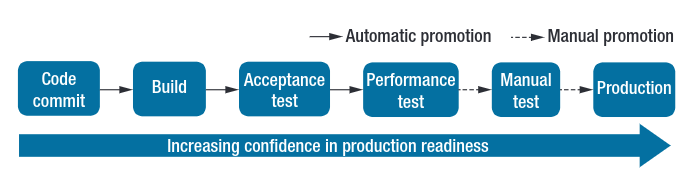
\includegraphics[width=1\textwidth]{images/continouse-delivery-pipeline.png}
    \caption{Contoh pipeline dalam Continous Delivery}
\end{figure}

\subsection{Metode Continuous Deployment}
Perbedaan mendasar dari Continuous Delivery (CDE) dan Continuous Deployment (CD) adalah dimana implementasi semua fase
dilakukan secara automatis tanpa memerlukan intervensi manusia, deployment
ke tahap environment produksi juga bisa dilakukan secara automatis, tetapi biasanya memerlukan intervensi pada satu tahap \cite{Ramadoni2021}.
\vspace{0.5cm}
\section{Deployment Pada Kubernetes}
Pada padasarnya terdapat 2 metode yang digunakan untuk melakukan
deployment pada sebuah aplikasi pada kubernetes yaitu pull method dan push method \cite{Ramadoni2021}.
Perbedaan  mendasar dari pull method dan push method terdapat pada agent yang melakukan
deployment \cite{GitOps}. Pada push method sebuah agent melakukan deployment sebuah  service terhadap suatu platform (eg, kubernetes).
\vspace{0.5cm}
\subsection{Push-based Deployment}
Push-based deployment \cite{GitOps} merupakan strategy yang popular yang diimplementasikan oleh
tools seperti Jenkins, CircleCI, atau TravisCI.
Sourcecode dari sebuah aplikasi terdapat pada repository yang sama dengan konfigurasi YAML Kubernetes yang diperlukan untuk melakukan deployment aplikasi tersebut.
Kapan pun code dari aplikasi tersebut diupdat, pipeline akan berjalan, dimana akan membuat container image yang diperlukan.
Perlu diperhatikan juga bahwa biasanya credential environment untuk melakukan deployment pada metode Push-based. Jadi pada pipeline tersebut kita dapat melihat
configurasi rahasia yang mungkin saja terlihat oleh orang lain.
\begin{figure}[ht]
    \centering
    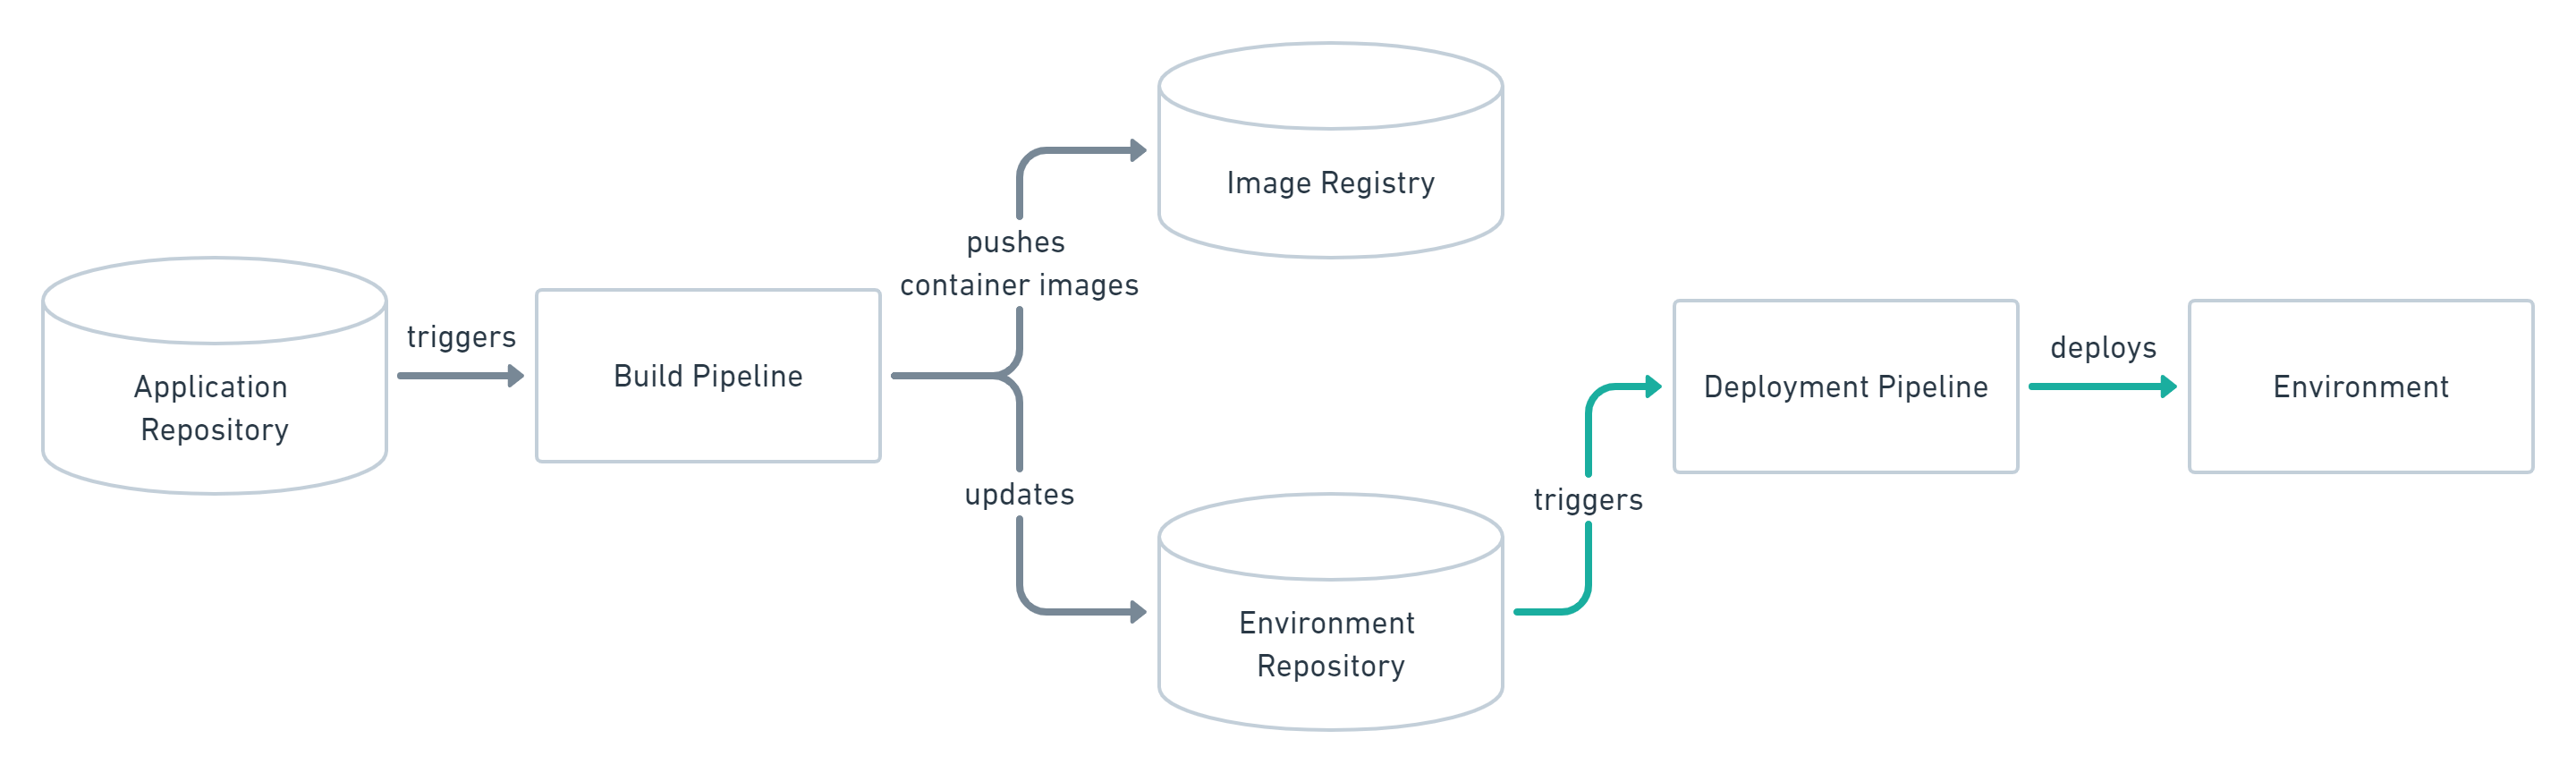
\includegraphics[width=1\textwidth]{images/push-based.png}
    \caption{Contoh pipeline dalam push-based deployment}
\end{figure}
\newpage
\vspace{0.5cm}
\subsection{Pull-based Deployment}
Pada website insert gitops Strategi Pull-based deployment menggunakan konsep
yang sama dengan push-based tetapi berbeda pada bagaimana cara kerja pada pipeline deployment.
Secara traditional pipeline CI/CD akan di-trigger oleh event eksternal, contohnya ketika ada update kode
baru yang pada repository. Dengan metode pull-based deployment, dikenalkan sebuah operator.
Operator tersebut secara kontinu dengan interval yang dapat diatur sendiri melakukan komparasi
terhadap state yang ada di repository dengan state yang ter-deploy pada infrastructure.
Ketika terdapat perbedaan, operator melakukan update pada infrastructure untuk mencocokan state dengan apa yang ada di repository.
Operator harus berada pada environment atau kluster yang sama dengan applikasi yang akan dideploy. Dengan ini pull-based method
tidak perlu mengetahui environment eksternal karena semua sudah ada pada kluster yang sama.
\begin{figure}[h]
    \centering
    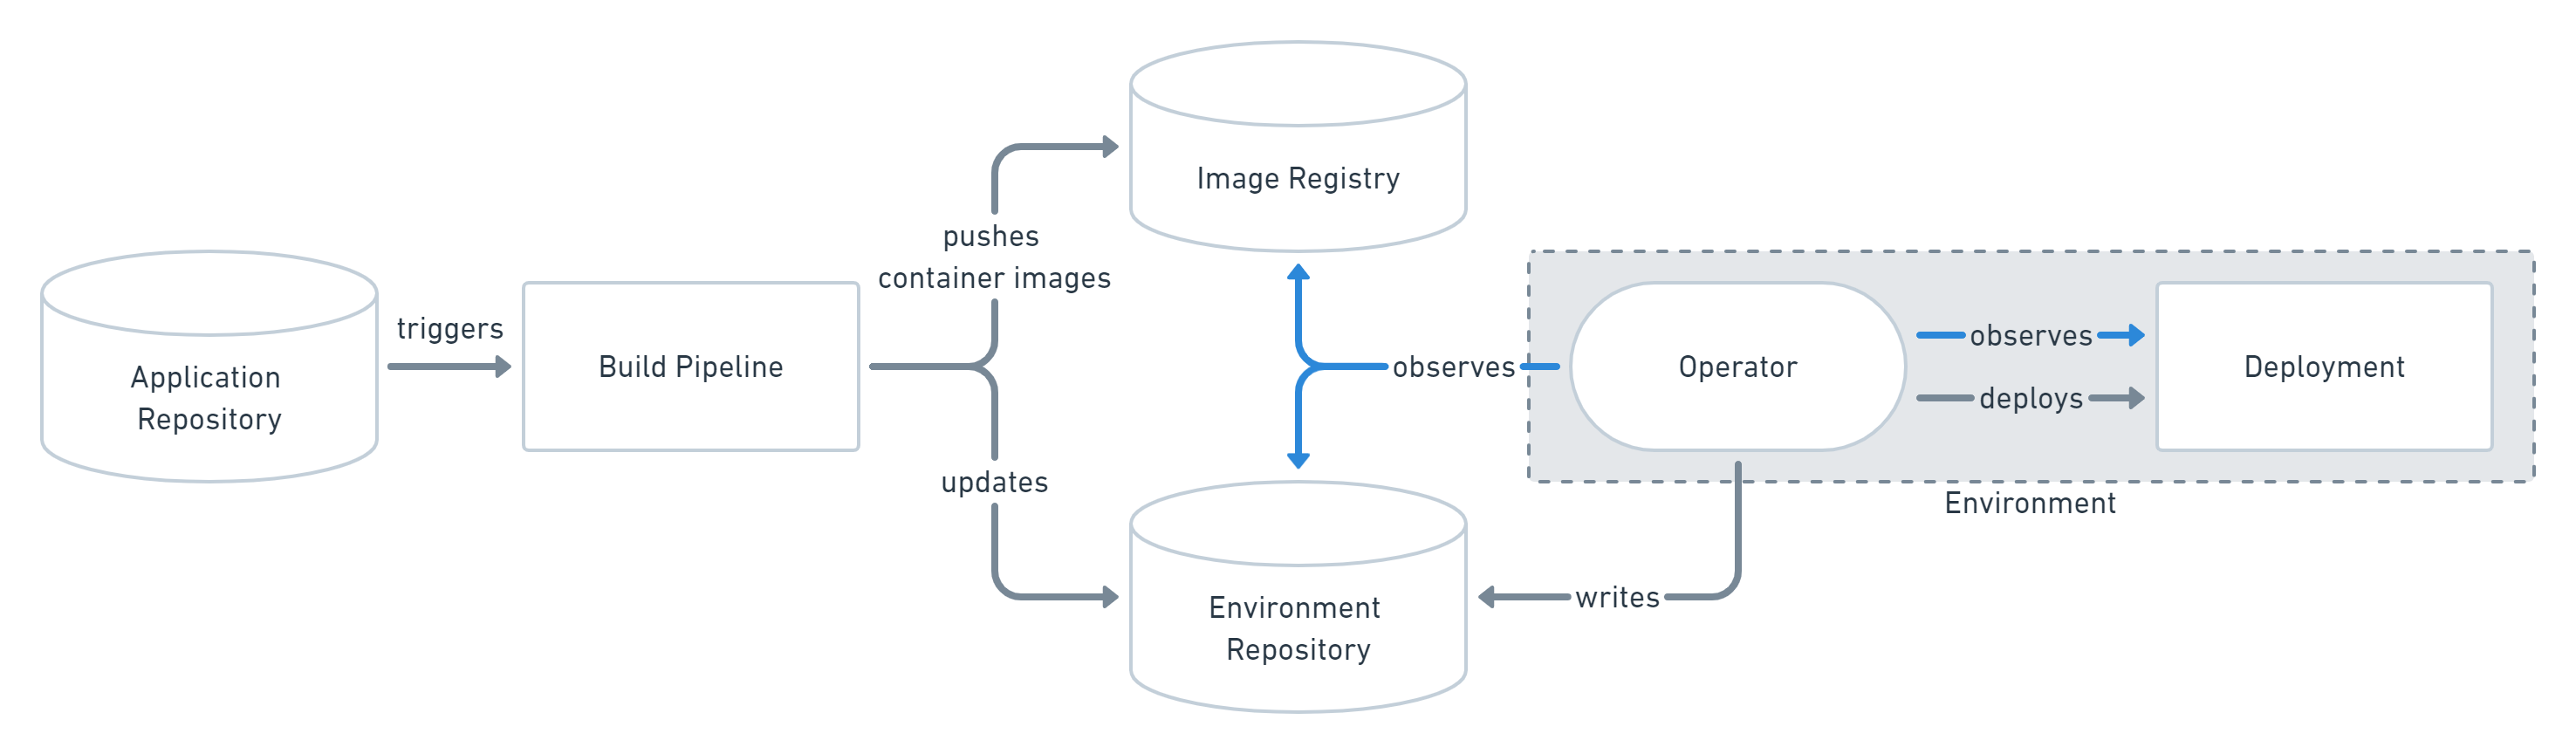
\includegraphics[width=1\textwidth]{images/pull-based.png}
    \caption{Contoh pipeline dalam pull-based deployment}
\end{figure}
\vspace{0.5cm}

\newpage
\section{Arsitektur Cluster Kubernetes yang akan digunakan}
Dibawah ini merupakan rancangan arsitektur high-level pada implementasi Kubernetes
nantinya. Disini menggunakan Metal-LB sebagai provider load  balancer dan Traefik sebagai ingress controller.
\begin{figure}[h]
    \centering
    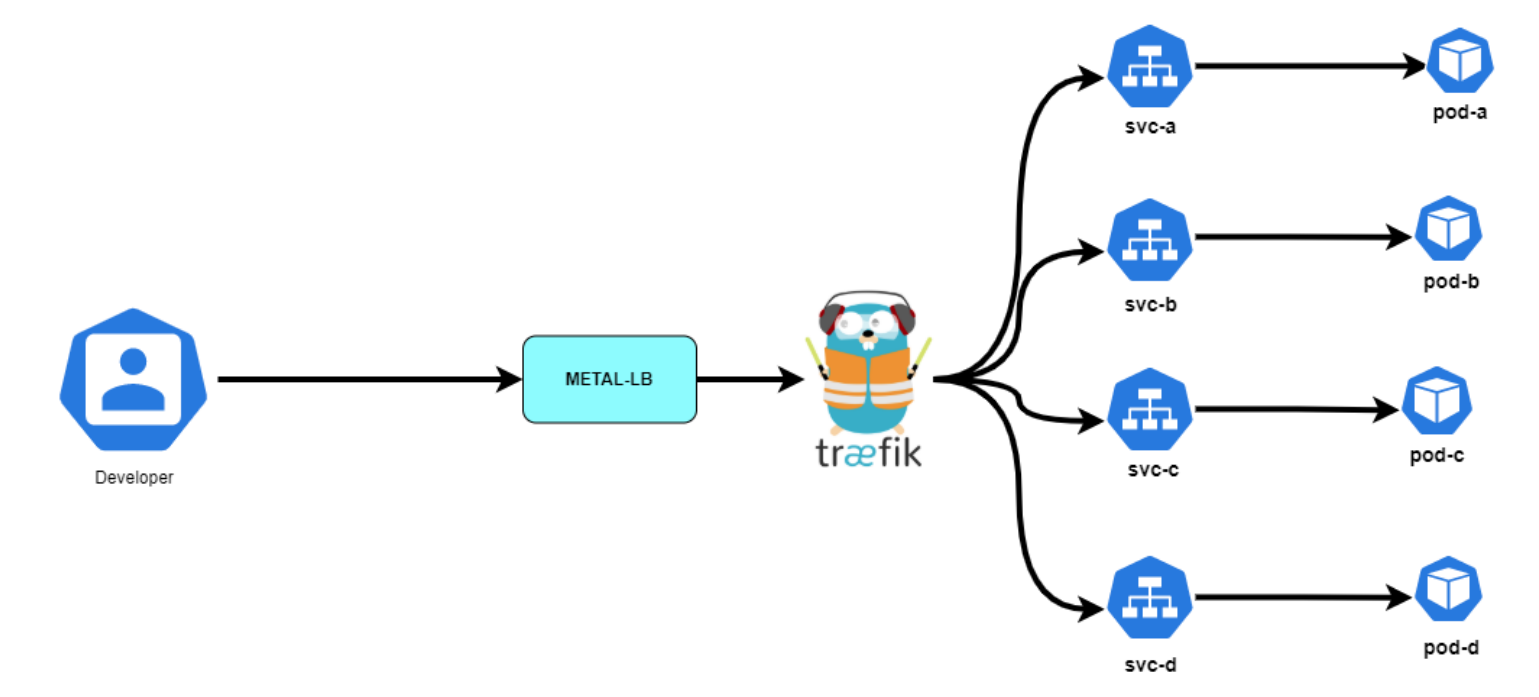
\includegraphics[width=1\textwidth]{images/kubernetes-arch.png}
    \caption{Arsitektur Kubernetes yang akan digunakan}
\end{figure}



% \section{Pengembangan Sistem}

% \section{Perangkat Lunak Pendukung}

% \begin{figure}[h]
%     \centering
%     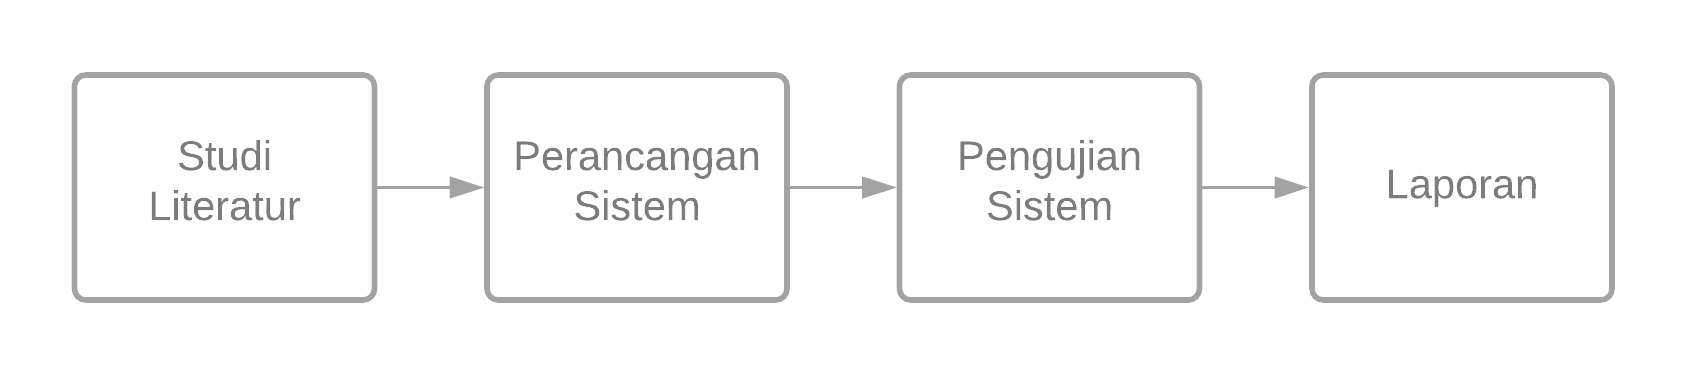
\includegraphics[width=0.9\textwidth]{images/timeline.png}
% \end{figure}
\newpage
%-----------------------------------------------------------------------------%
\chapter{KESIMPULAN}
%-----------------------------------------------------------------------------%

%
\vspace{4.5pt}
Deployment software berbasis microservice saat ini banyak menggunakan
container dan dibutuhkan kubernetes untuk melakukan orkestrasi container-container tersebut.
Deployment sistem terdistribusi khususnya pada platform kubernetes cukuplah kompleks.
Cepatnya perubahan dan meningkatnya  kompleksitas sebuah software yang dikembangkan dibutuhkan
suatu cara untuk  melakukan deployment secara automatis agar seorang developer dapat  mendapatkan
feedback secara cepat tentang apa yang dikerjakannya.
Oleh karena itu diperlukan penerapan Continous Deployment yang mengikuti prinsip GitOps akan didapatkan produktifitas tinggi dari sisi developer dan management.
% %-----------------------------------------------------------------------------%
\chapter{IMPLEMENTASI DAN PENGUJIAN}
%-----------------------------------------------------------------------------%

%
\vspace{4.5pt}

\section{Implementasi}

\subsection{Lingkungan Perangkat Lunak}

\subsection{Spesifikasi Perangkat Keras}

\subsection{Impelementasi Antarmuka}

\subsubsection{Impelementasi Halaman Utama}

\subsubsection{Implementasi Menu File}

\subsubsection{Implementasi Menu}

\subsection{Pengguna Program}

\section{Pengujian}

\subsection{Pengujian Blackbox}

\subsection{Pengujian Whitebox}

\newpage
% %-----------------------------------------------------------------------------%
\chapter{PENUTUP}
%-----------------------------------------------------------------------------%

%
\vspace{4.5pt}

\section{Kesimpulan}

\subsection{Saran}

\newpage

% Merubah Nama Bibliografi ke Daftar Pustaka
\renewcommand{\bibname}{DAFTAR PUSTAKA}
\phantomsection
\addcontentsline{toc}{chapter}{DAFTAR PUSTAKA}
% Daftar Pustaka
\bibliographystyle{IEEEtranN}
\bibliography{export}
% %
% Daftar Pustaka 
% 
%Format Penulisan Daftar Pustaka yang di Sesuai dengan aturan penulisan Unair
%==========================================================================================
%\bibitem[Nama,tahun]{citasi}
%Nama Pengarang, Tahun,
%\newblock \emph{Judul dan keterangan}.
%\newblock Penerbit, Kota.
%========================================================================================== 
% Tambahkan pustaka yang digunakan setelah perintah berikut. 
% 
\begin{thebibliography}{7}
%\bibliographystyle{unsrt}
\providecommand{\natexlab}[1]{#1}
\providecommand{\url}[1]{\texttt{#1}}
\expandafter\ifx\csname urlstyle\endcsname\relax
  \providecommand{\doi}[1]{doi: #1}\else
  \providecommand{\doi}{doi: \begingroup \urlstyle{rm}\Url}\fi

\bibitem[Akbar,2008]{taufik}
Akbar, T, 2008,
\newblock \emph{Penentuan Spektrum Aksi \textit{Porphyrin} Dengan Metode
  Semi-Empirik \textit{Hartree-Fock} (Skripsi)}.
\newblock Departemen Fisika, Universitas Airlangga.

\bibitem[Arias,2005]{arias}
Arias.T.A, 2005,
\newblock Notes on the ab initio theory of molecules and solids: Density
  functional theory (dft).
\newblock Cornell University.

\bibitem[Darmawan,2009]{darmawan}
Darmawan, E, 2009,
\newblock \emph{Pemrograman Dasar C-Java-C\#}.
\newblock Penerbit Informatika, Bandung.

\bibitem[Haken,1994]{haken}
Haken, Hermann. W.C, 1994,
\newblock \emph{{M}olecular {P}hysics and {E}lements of {Q}uantum {C}hemistry}.
\newblock Springer. USA

\bibitem[Hiroshi,2009]{hiroshi}
Hiroshi Katayama-Yoshida, 2009,
\newblock Computational Nano-Materials Design for Spinodal Nanotechnology.
\newblock Osaka University Japan

\bibitem[Rinaldi,2008]{munir}
Rinaldi. M, 2008,
\newblock \emph{Metode Numerik}.
\newblock Penerbit Informatika, Bandung

\bibitem[Siregar,2010]{rustam}
Siregar. R.E, 2010,
\newblock \emph{Teori dan Aplikasi Fisika Kuantum}.
\newblock Widya Padjadjaran, Bandung.

\bibitem[S.S.~David,2009]{david}
Shols.~David,S .A.~J, 2009,
\newblock \emph{{D}ENSITY {F}UNCTIONAL {T}HEORY A {P}ractical {I}ntroduction}.
\newblock John Wiley and Sons, Inc,

\bibitem[William H.~Press,1999]{william}
S.~A.~T. William H.~Press, Brian P.~Flannery, 1999, 
\newblock \emph{{N}umerical {R}ecipes in {C}. {T}he {A}rt of {S}cientific
  {C}omputing}.
\newblock Cambridge University Press.


\bibitem[NIST(2011)]{nist}
http://physics.nist.gov/PhysRefData/DFTdata.
\newblock Atomic Reference Data for Electron Structure Calculation.
\newblock 08 Februari 2011.


\end{thebibliography}



%
% Lampiran 
%

\setcounter{originalpagenumber}{\number\value{page}}%
\setcounter{page}{0}
\pagenumbering{arabic}

\onehalfspacing
% \begin{appendix}
% %
% @author  Andreas Febrian
% @version 1.00 
% 
% Hanya sebuah pembatas bertuliskan LAMPIRAN ditengah halaman. 
% 

\begin{titlepage}
	\centering 
	\vspace*{6cm}
	\noindent \Huge{LAMPIRAN}
\end{titlepage}
% \end{appendix}

\pagenumbering{arabic}% 
\setcounter{page}{\number\value{originalpagenumber}}
\clearpage
% \phantomsection \addcontentsline{toc}{chapter}{LAMPIRAN}
% 
%-----------------------------------------------------------------------------%
\section*{Coding Login Aplikasi}
%-----------------------------------------------------------------------------%



\end{document}